\documentclass{standalone}
\usepackage{tikz}
\usetikzlibrary{patterns, positioning}
\usepackage[sfdefault]{ClearSans} %% option 'sfdefault' activates Clear Sans as the default text font
\usepackage[T1]{fontenc}

\begin{document}
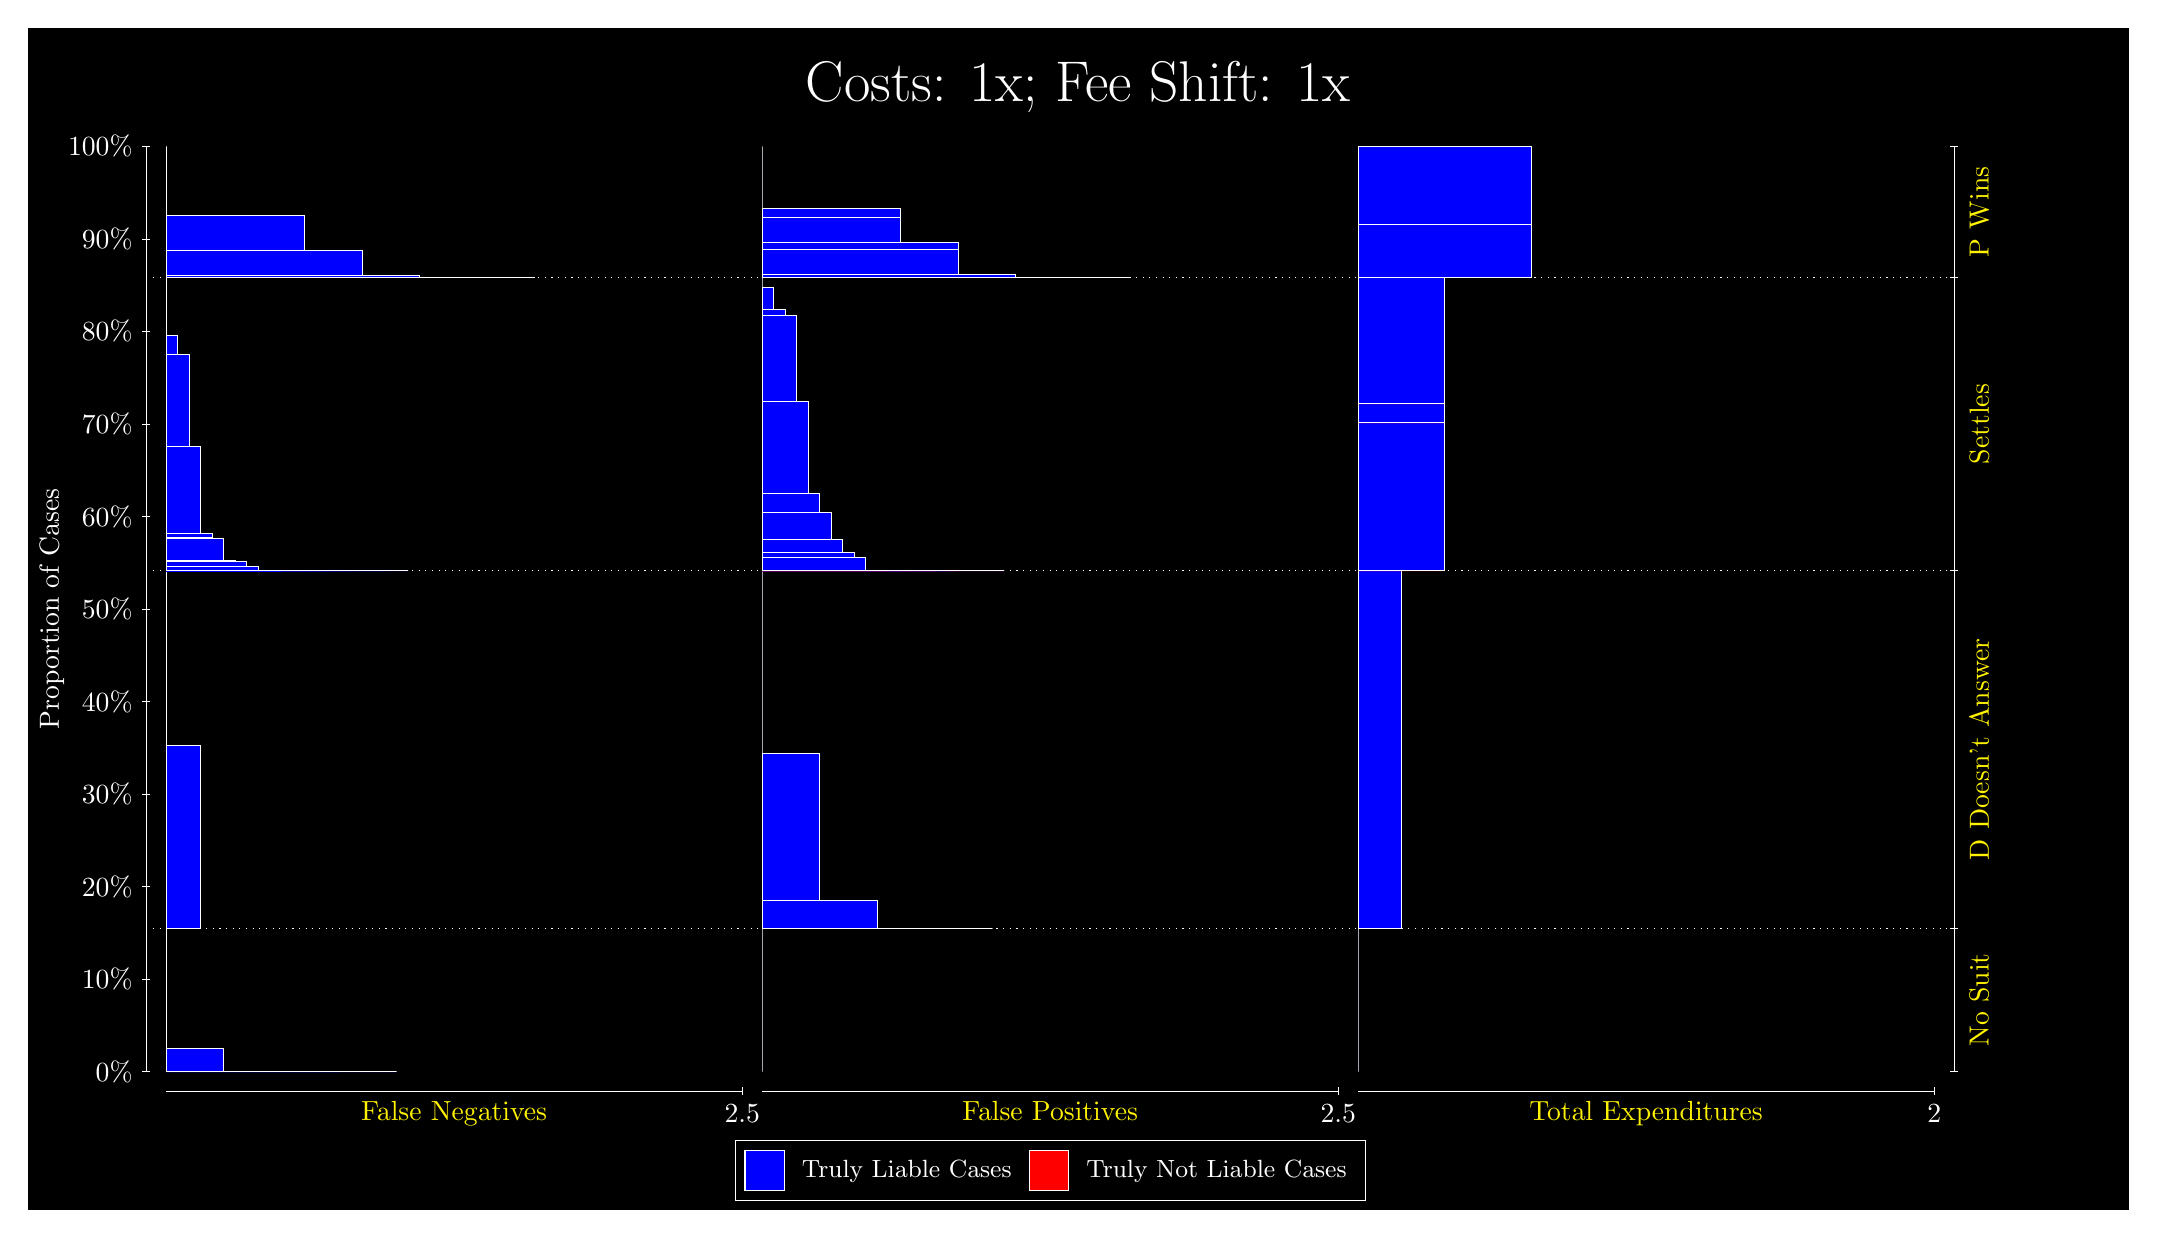
\begin{tikzpicture}
\draw[fill=black] (0,0) rectangle (26.667,15);
\draw[text=white] (0,13.5) rectangle (26.667,15) node[midway] {\huge Costs: 1x; Fee Shift: 1x};
\draw[white, very thin] (1.5,1.75) -- (1.5,13.5);
\node[rotate=90, text=white, anchor=center] at (0.3, 7.625) {Proportion of Cases};
\draw[white, very thin] (1.45,1.75) -- (1.55,1.75);
\node[text=white, anchor=east] at (1.45, 1.75) {0\%};
\draw[white, very thin] (1.45,2.925) -- (1.55,2.925);
\node[text=white, anchor=east] at (1.45, 2.925) {10\%};
\draw[white, very thin] (1.45,4.1) -- (1.55,4.1);
\node[text=white, anchor=east] at (1.45, 4.1) {20\%};
\draw[white, very thin] (1.45,5.275) -- (1.55,5.275);
\node[text=white, anchor=east] at (1.45, 5.275) {30\%};
\draw[white, very thin] (1.45,6.45) -- (1.55,6.45);
\node[text=white, anchor=east] at (1.45, 6.45) {40\%};
\draw[white, very thin] (1.45,7.625) -- (1.55,7.625);
\node[text=white, anchor=east] at (1.45, 7.625) {50\%};
\draw[white, very thin] (1.45,8.8) -- (1.55,8.8);
\node[text=white, anchor=east] at (1.45, 8.8) {60\%};
\draw[white, very thin] (1.45,9.975) -- (1.55,9.975);
\node[text=white, anchor=east] at (1.45, 9.975) {70\%};
\draw[white, very thin] (1.45,11.15) -- (1.55,11.15);
\node[text=white, anchor=east] at (1.45, 11.15) {80\%};
\draw[white, very thin] (1.45,12.325) -- (1.55,12.325);
\node[text=white, anchor=east] at (1.45, 12.325) {90\%};
\draw[white, very thin] (1.45,13.5) -- (1.55,13.5);
\node[text=white, anchor=east] at (1.45, 13.5) {100\%};

\draw[white, very thin] (24.457,1.75) -- (24.457,13.5);
\draw[white, very thin] (24.407,1.75) -- (24.507,1.75);
\node[anchor=west] at (24.407, 1.75) {};
\draw[white, very thin] (24.407,3.5712) -- (24.507,3.5712);
\node[anchor=west] at (24.407, 3.5712) {};
\draw[white, very thin] (24.407,8.1102) -- (24.507,8.1102);
\node[anchor=west] at (24.407, 8.1102) {};
\draw[white, very thin] (24.407,11.836) -- (24.507,11.836);
\node[anchor=west] at (24.407, 11.836) {};
\draw[white, very thin] (24.407,13.5) -- (24.507,13.5);
\node[anchor=west] at (24.407, 13.5) {};

\draw[white, very thin, fill=blue] (1.75,1.75) rectangle (4.6775,1.75);
\draw[white, very thin, fill=blue] (1.75,1.75) rectangle (3.9457,1.75);
\draw[white, very thin, fill=blue] (1.75,1.75) rectangle (3.2138,1.7525);
\draw[white, very thin, fill=blue] (1.75,1.7525) rectangle (2.4819,2.0482);
\draw[white, very thin, fill=red] (1.75,2.0482) rectangle (1.75,2.0482);
\draw[white, very thin, fill=blue] (1.75,2.0482) rectangle (1.75,3.5712);
\draw[white, very thin, fill=blue] (1.75,3.5712) rectangle (2.1891,5.8885);
\draw[white, very thin, fill=red] (1.75,5.8885) rectangle (1.75,5.8885);
\draw[white, very thin, fill=blue] (1.75,5.8885) rectangle (1.75,8.1102);
\draw[white, very thin, fill=blue] (1.75,8.1102) rectangle (4.8239,8.1102);
\draw[white, very thin, fill=blue] (1.75,8.1102) rectangle (4.5312,8.1102);
\draw[white, very thin, fill=blue] (1.75,8.1102) rectangle (4.2384,8.1102);
\draw[white, very thin, fill=blue] (1.75,8.1102) rectangle (4.092,8.1102);
\draw[white, very thin, fill=blue] (1.75,8.1102) rectangle (3.9457,8.1102);
\draw[white, very thin, fill=blue] (1.75,8.1102) rectangle (3.7993,8.1102);
\draw[white, very thin, fill=blue] (1.75,8.1102) rectangle (3.6529,8.1102);
\draw[white, very thin, fill=blue] (1.75,8.1102) rectangle (3.5065,8.1102);
\draw[white, very thin, fill=blue] (1.75,8.1102) rectangle (3.3602,8.1102);
\draw[white, very thin, fill=blue] (1.75,8.1102) rectangle (3.2138,8.1107);
\draw[white, very thin, fill=blue] (1.75,8.1107) rectangle (3.0674,8.1108);
\draw[white, very thin, fill=blue] (1.75,8.1108) rectangle (3.0674,8.1109);
\draw[white, very thin, fill=blue] (1.75,8.1109) rectangle (2.921,8.1699);
\draw[white, very thin, fill=blue] (1.75,8.1699) rectangle (2.7746,8.2287);
\draw[white, very thin, fill=blue] (1.75,8.2287) rectangle (2.6283,8.2288);
\draw[white, very thin, fill=blue] (1.75,8.2288) rectangle (2.6283,8.2377);
\draw[white, very thin, fill=blue] (1.75,8.2377) rectangle (2.4819,8.5189);
\draw[white, very thin, fill=blue] (1.75,8.5189) rectangle (2.3355,8.5357);
\draw[white, very thin, fill=blue] (1.75,8.5357) rectangle (2.3355,8.5896);
\draw[white, very thin, fill=blue] (1.75,8.5896) rectangle (2.1891,9.6856);
\draw[white, very thin, fill=blue] (1.75,9.6856) rectangle (2.0428,10.858);
\draw[white, very thin, fill=blue] (1.75,10.858) rectangle (1.8964,10.862);
\draw[white, very thin, fill=blue] (1.75,10.862) rectangle (1.8964,11.096);
\draw[white, very thin, fill=red] (1.75,11.096) rectangle (1.75,11.096);
\draw[white, very thin, fill=blue] (1.75,11.096) rectangle (1.75,11.836);
\draw[white, very thin, fill=blue] (1.75,11.836) rectangle (6.4341,11.836);
\draw[white, very thin, fill=blue] (1.75,11.836) rectangle (5.7022,11.837);
\draw[white, very thin, fill=blue] (1.75,11.837) rectangle (4.9703,11.857);
\draw[white, very thin, fill=blue] (1.75,11.857) rectangle (4.2384,12.178);
\draw[white, very thin, fill=blue] (1.75,12.178) rectangle (3.9457,12.178);
\draw[white, very thin, fill=blue] (1.75,12.178) rectangle (3.5065,12.622);
\draw[white, very thin, fill=blue] (1.75,12.622) rectangle (3.2138,12.622);
\draw[white, very thin, fill=blue] (1.75,12.622) rectangle (2.7746,12.622);
\draw[white, very thin, fill=blue] (1.75,12.622) rectangle (2.4819,12.625);
\draw[white, very thin, fill=blue] (1.75,12.625) rectangle (2.0428,12.625);
\draw[white, very thin, fill=red] (1.75,12.625) rectangle (1.75,12.625);
\draw[white, very thin, fill=blue] (1.75,12.625) rectangle (1.75,13.5);
\draw[white, very thin, fill=red] (9.3189,1.75) rectangle (9.3189,1.75);
\draw[white, very thin, fill=blue] (9.3189,1.75) rectangle (9.3189,3.5712);
\draw[white, very thin, fill=red] (9.3189,3.5712) rectangle (12.246,3.5712);
\draw[white, very thin, fill=blue] (9.3189,3.5712) rectangle (12.246,3.5712);
\draw[white, very thin, fill=blue] (9.3189,3.5712) rectangle (11.515,3.5738);
\draw[white, very thin, fill=blue] (9.3189,3.5738) rectangle (10.783,3.922);
\draw[white, very thin, fill=blue] (9.3189,3.922) rectangle (10.051,5.793);
\draw[white, very thin, fill=blue] (9.3189,5.793) rectangle (9.3189,8.1102);
\draw[white, very thin, fill=red] (9.3189,8.1102) rectangle (12.393,8.1102);
\draw[white, very thin, fill=blue] (9.3189,8.1102) rectangle (12.393,8.1102);
\draw[white, very thin, fill=red] (9.3189,8.1102) rectangle (11.807,8.1102);
\draw[white, very thin, fill=blue] (9.3189,8.1102) rectangle (11.807,8.1102);
\draw[white, very thin, fill=blue] (9.3189,8.1102) rectangle (11.661,8.1102);
\draw[white, very thin, fill=red] (9.3189,8.1102) rectangle (11.515,8.1102);
\draw[white, very thin, fill=blue] (9.3189,8.1102) rectangle (11.515,8.1102);
\draw[white, very thin, fill=red] (9.3189,8.1102) rectangle (11.222,8.1102);
\draw[white, very thin, fill=blue] (9.3189,8.1102) rectangle (11.222,8.1102);
\draw[white, very thin, fill=blue] (9.3189,8.1102) rectangle (11.075,8.1102);
\draw[white, very thin, fill=red] (9.3189,8.1102) rectangle (10.929,8.1102);
\draw[white, very thin, fill=blue] (9.3189,8.1102) rectangle (10.929,8.1148);
\draw[white, very thin, fill=blue] (9.3189,8.1148) rectangle (10.783,8.1149);
\draw[white, very thin, fill=red] (9.3189,8.1149) rectangle (10.636,8.1149);
\draw[white, very thin, fill=blue] (9.3189,8.1149) rectangle (10.636,8.2852);
\draw[white, very thin, fill=blue] (9.3189,8.2852) rectangle (10.49,8.3436);
\draw[white, very thin, fill=red] (9.3189,8.3436) rectangle (10.344,8.3436);
\draw[white, very thin, fill=blue] (9.3189,8.3436) rectangle (10.344,8.5084);
\draw[white, very thin, fill=blue] (9.3189,8.5084) rectangle (10.197,8.8502);
\draw[white, very thin, fill=red] (9.3189,8.8502) rectangle (10.051,8.8502);
\draw[white, very thin, fill=blue] (9.3189,8.8502) rectangle (10.051,9.089);
\draw[white, very thin, fill=blue] (9.3189,9.089) rectangle (9.9044,10.261);
\draw[white, very thin, fill=blue] (9.3189,10.261) rectangle (9.758,11.357);
\draw[white, very thin, fill=blue] (9.3189,11.357) rectangle (9.6116,11.428);
\draw[white, very thin, fill=blue] (9.3189,11.428) rectangle (9.4652,11.709);
\draw[white, very thin, fill=blue] (9.3189,11.709) rectangle (9.3189,11.836);
\draw[white, very thin, fill=red] (9.3189,11.836) rectangle (14.003,11.836);
\draw[white, very thin, fill=blue] (9.3189,11.836) rectangle (14.003,11.836);
\draw[white, very thin, fill=red] (9.3189,11.836) rectangle (13.271,11.836);
\draw[white, very thin, fill=blue] (9.3189,11.836) rectangle (13.271,11.837);
\draw[white, very thin, fill=red] (9.3189,11.837) rectangle (12.539,11.837);
\draw[white, very thin, fill=blue] (9.3189,11.837) rectangle (12.539,11.869);
\draw[white, very thin, fill=blue] (9.3189,11.869) rectangle (11.807,12.192);
\draw[white, very thin, fill=red] (9.3189,12.192) rectangle (11.807,12.192);
\draw[white, very thin, fill=blue] (9.3189,12.192) rectangle (11.807,12.276);
\draw[white, very thin, fill=blue] (9.3189,12.276) rectangle (11.075,12.593);
\draw[white, very thin, fill=blue] (9.3189,12.593) rectangle (11.075,12.712);
\draw[white, very thin, fill=red] (9.3189,12.712) rectangle (10.783,12.712);
\draw[white, very thin, fill=blue] (9.3189,12.712) rectangle (10.783,12.712);
\draw[white, very thin, fill=blue] (9.3189,12.712) rectangle (10.344,12.714);
\draw[white, very thin, fill=blue] (9.3189,12.714) rectangle (10.344,12.714);
\draw[white, very thin, fill=red] (9.3189,12.714) rectangle (10.051,12.714);
\draw[white, very thin, fill=blue] (9.3189,12.714) rectangle (10.051,12.715);
\draw[white, very thin, fill=blue] (9.3189,12.715) rectangle (9.6116,12.715);
\draw[white, very thin, fill=blue] (9.3189,12.715) rectangle (9.6116,12.715);
\draw[white, very thin, fill=red] (9.3189,12.715) rectangle (9.3189,12.715);
\draw[white, very thin, fill=blue] (9.3189,12.715) rectangle (9.3189,13.5);
\draw[white, very thin, fill=red] (16.888,1.75) rectangle (16.888,1.75);
\draw[white, very thin, fill=blue] (16.888,1.75) rectangle (16.888,3.5712);
\draw[white, very thin, fill=red] (16.888,3.5712) rectangle (17.437,3.5712);
\draw[white, very thin, fill=blue] (16.888,3.5712) rectangle (17.437,8.1102);
\draw[white, very thin, fill=red] (16.888,8.1102) rectangle (17.986,8.1102);
\draw[white, very thin, fill=blue] (16.888,8.1102) rectangle (17.986,9.9894);
\draw[white, very thin, fill=red] (16.888,9.9894) rectangle (17.986,9.9894);
\draw[white, very thin, fill=blue] (16.888,9.9894) rectangle (17.986,10.233);
\draw[white, very thin, fill=red] (16.888,10.233) rectangle (17.986,10.233);
\draw[white, very thin, fill=blue] (16.888,10.233) rectangle (17.986,11.836);
\draw[white, very thin, fill=red] (16.888,11.836) rectangle (19.083,11.836);
\draw[white, very thin, fill=blue] (16.888,11.836) rectangle (19.083,12.511);
\draw[white, very thin, fill=red] (16.888,12.511) rectangle (19.083,12.511);
\draw[white, very thin, fill=blue] (16.888,12.511) rectangle (19.083,13.5);
\draw[white, dotted] (1.5,3.5712) -- (24.457,3.5712);
\draw[white, dotted] (1.5,8.1102) -- (24.457,8.1102);
\draw[white, dotted] (1.5,11.836) -- (24.457,11.836);
\draw[white, very thin] (1.75,1.5) -- (9.0689,1.5);
\node[text=yellow, anchor=north] at (5.4094, 1.5) {False Negatives};
\draw[white, very thin] (9.0689,1.45) -- (9.0689,1.55);
\node[text=white, anchor=north] at (9.0689, 1.45) {2.5};

\draw[white, very thin] (9.3189,1.5) -- (16.638,1.5);
\node[text=yellow, anchor=north] at (12.978, 1.5) {False Positives};
\draw[white, very thin] (16.638,1.45) -- (16.638,1.55);
\node[text=white, anchor=north] at (16.638, 1.45) {2.5};

\draw[white, very thin] (16.888,1.5) -- (24.207,1.5);
\node[text=yellow, anchor=north] at (20.547, 1.5) {Total Expenditures};
\draw[white, very thin] (24.207,1.45) -- (24.207,1.55);
\node[text=white, anchor=north] at (24.207, 1.45) {2};

\node[text=yellow, centered, rotate=90] at (24.777, 2.6606) {No Suit};
\node[text=yellow, centered, rotate=90] at (24.777, 5.8407) {D Doesn't Answer};
\node[text=yellow, centered, rotate=90] at (24.777, 9.9733) {Settles};
\node[text=yellow, centered, rotate=90] at (24.777, 12.668) {P Wins};

\draw (12.978300999999998,1.5) node[draw=none] (baseCoordinate) {};
\begin{scope}[align=center]
        \matrix[scale=0.5, draw=white, below=0.5cm of baseCoordinate, nodes={draw}, column sep=0.1cm]{
            \node[rectangle, draw, minimum width=0.5cm, minimum height=0.5cm, fill=blue] {}; &
            \node[draw=none, font=\small, text=white] (B) {Truly Liable Cases}; &
            \node[rectangle, draw, minimum width=0.5cm, minimum height=0.5cm, fill=red] {}; &
            \node[draw=none, font=\small, text=white] (B) {Truly Not Liable Cases}; \\
            };
\end{scope}

\end{tikzpicture}
\end{document}